\documentclass[12pt]{report}
\usepackage[utf8]{inputenc}
\usepackage{xcolor}
\usepackage[margin=1in]{geometry}
\usepackage{soul} 
\usepackage{apacite}
\usepackage{graphicx}
\usepackage{xurl}
\usepackage{subcaption}
\usepackage{amsmath}
\captionsetup{compatibility=false}

\usepackage{fancyhdr}
\pagestyle{fancy}

\lhead{Research Project}
\rhead{Draft}
\cfoot{\thepage}
\renewcommand{\headrulewidth}{0.4pt}
\renewcommand{\footrulewidth}{0.4pt}

\title{Parameterizing Play:\\ Exploring Game Dynamics in Snakes and Ladders}
\author{Jai Bakshi \\ 21060322069}
\date{February 2025}

\begin{document}
	\maketitle
	\chapter{Introduction}
	From the simple delight of childhood board games to the intricate strategies of modern tabletop experiences, games hold a fundamental appeal for humanity. As Peter Gray (2017)  argues, play is not merely frivolous pastime but a powerful vehicle for learning and development, deeply ingrained in our nature. Games, in their essence, are structured systems that invite players to engage in artificial conflicts governed by predefined rules, ultimately leading to quantifiable outcomes (Puentedura, n.d.). This act of play, this engagement within a rule-bound system, is where the potential for enjoyment resides. Understanding and quantifying this ‘enjoyment’ becomes a complex undertaking. It is influenced by a myriad of factors, ranging from individual preferences and social dynamics to the inherent design and mechanics of the game itself. In the context of game studies and design, it becomes crucial to move beyond subjective impressions and explore methods to systematically analyse and potentially quantify the elements that contribute to a game's enjoyability.
	
	This dissertation focuses on the specific domain of table-top games – a rich and tangible space for exploring game mechanics and player interaction. Tabletop games, encompassing board games, card games, and dice games, offer a unique lens through which to examine the relationship between game design and player experience. Their tangible nature, the direct manipulation of components, and the face-to-face social interaction create a particularly fertile ground for investigating the sources of game enjoyment. Within this exploration, one must consider the philosophical underpinnings of what constitutes a game. Bernard Suits, in his seminal work The Grasshopper: Games, Life and Utopia (1978), provides a valuable framework. Suits introduces the concept of the ``lusory attitude,'' the willing acceptance of constitutive rules to engage in activity aimed at achieving a specific state of affairs (the lusory goal), where such rules prohibit the most efficient means of achieving that state. This ``lusory attitude'' is central to understanding games as distinct from ordinary life, operating within what Johan Huizinga termed the ``magic circle''—a bounded space where different rules and expectations apply. By embracing this perspective, one can begin to dissect the intricate relationship between game mechanics, player engagement, and the elusive quality of enjoyability. This research,  will distinguish between two key aspects of game enjoyment: mechanical enjoyability – the enjoyment derived from the inherent design and mechanics of the game system itself, and experiential enjoyability – the fluctuating enjoyment stemming from player decisions, social interactions, and the unfolding narrative of a particular game session.
	
	\section{Moving Beyond Subjectivity}
	While the allure of games is universally acknowledged, the nature of enjoyment itself remains inherently subjective. As Nicole Lazzaro (2004) emphasizes in her examination of “Four Keys to More Emotion Without Story,” factors like social interaction (``People Factor'') and individual player preferences significantly shape the overall gaming experience. Consequently, assessing game enjoyability is not as straightforward as evaluating objective features. Existing game review systems, as analysed by Yang and Mei (2010), often grapple with this subjectivity. These systems, while providing valuable consumer feedback, are inherently limited by their reliance on subjective opinions and the tendency to focus on “search attributes” – features readily apparent before playing – rather than “experiential attributes” – those felt only through gameplay. Furthermore, Yang and Mei’s research reveals that negative reviews can disproportionately influence perceptions, and the network effect, where shared experiences amplify enjoyment (or dissatisfaction), further complicates objective assessment.
	
	This inherent subjectivity does not negate the need for a more systematic and potentially quantifiable approach to understanding game enjoyment. Indeed, to advance game design and analysis, one must strive to bridge the gap between subjective experience and objective analysis. This research affirms that while experiential enjoyability remains inherently variable, mechanical enjoyability, rooted in the game's core mechanics, can be approached as a more quantifiable construct. By focusing on the design elements and rule systems that structure gameplay, this project aims to develop methods for objectively assessing and potentially predicting the level of enjoyment a game's mechanics might elicit.
	
	\section{Snakes and Ladders: A timeless classic}
	To ground our exploration of game enjoyability in a tangible example, this dissertation will reference the game of Snakes and Ladders. As Marcus du Sautoy (2023) might illuminate in his works exploring the mathematical underpinnings of games, Snakes and Ladders is far from being a trivial childhood pastime; it boasts a rich history and a remarkable universality that makes it an ideal case study for understanding fundamental game mechanics and player engagement.  Its origins can be traced back to ancient India, where it was known as \textit{Moksha Patam} or \textit{Gyan Chaupar}.  Reflecting insights often found in du Sautoy's discussions on the history of games and the mathematics surrounding them, this game, believed to have emerged as early as the 2nd century BC, was not merely entertainment but served as a moral and didactic tool. The ladders represented virtues like generosity, faith, and humility, while the snakes symbolized vices such as lust, anger, theft, and pride.  The ascent and descent on the board mirrored the karmic cycle of life, illustrating the consequences of good and bad actions in a visually compelling and accessible way.
	
	Over centuries, \textit{Moksha Patam} traveled beyond India, evolving and adapting as it spread across cultures, a journey that resonates with du Sautoy's broader narratives of how ideas and concepts traverse geographical and cultural boundaries. By the late 19th century, a Westernized version, "Snakes and Ladders," emerged in England and quickly gained popularity worldwide. While the overt moralistic undertones diminished in its global iteration, the core mechanics of chance, progression, setbacks, and the simple pursuit of a defined goal remained intact.  This enduring appeal across diverse cultures and time periods, echoing themes of universality often explored by du Sautoy in mathematical and historical contexts, underscores the game's ability to tap into fundamental aspects of human engagement and enjoyment.
	
	Snakes and Ladders, in its simplicity, offers a microcosm of the broader challenges in quantifying game enjoyability.  Its mechanics are easily grasped – the roll of a die dictates movement, and predetermined snakes and ladders introduce elements of both fortune and misfortune.  Yet, even within this seemingly straightforward system, players experience a range of emotions: anticipation with each dice roll, frustration upon encountering a snake, elation when climbing a ladder, and the ultimate satisfaction of reaching the final square.  The game’s accessibility and widespread familiarity make it an excellent lens through which to examine how even basic game mechanics, governed by chance and simple rules, can generate engaging and emotionally resonant player experiences. By analyzing Snakes and Ladders through the framework of mechanical and experiential enjoyability, one can begin to isolate and understand the core design elements that contribute to the enduring appeal of tabletop games, and potentially, games more broadly.
	
	\chapter{The Dynamics of Snakes and Ladders}
	This chapter delves into the mechanics of the classic game \textit{Snakes and Ladders}, aiming to quantify the impact of various game parameters on the overall game dynamics. This is achieved by simulating numerous games while systematically varying parameters. In this chapter, we will investigate two key aspects: firstly, the impact of the \textit{number} of snakes and ladders on the board, and secondly, the effects of varying the \textit{lengths} of these entities. To simplify the analysis and isolate the effects of these parameters, the model reduces the game to its essential elements. This allows us to systematically examine how changes in these parameters affect the distribution of game duration – specifically, the number of moves needed to reach the end state. This distinction in parameter variability helps separate the core game mechanics from the broader gameplay experience.
	
	\section{Setting up the board}
	
	In our pilot study, the game board is modelled as a 10x10 grid, comprising 100 squares, akin to the classic Snakes and Ladders game. The player, represented by an Agent in our model, starts at tile 1, with no requirement to roll a specific number to begin (i.e., no starting condition). The goal state is to reach or exceed tile 100. The Agent's movement is determined by a fair six-sided die roll.
	
	To facilitate a systematic investigation of game dynamics, this research introduces several controllable parameters that define the entities on the board:
	
	\begin{enumerate}
		\item \textbf{Board Size }($BoardSize$): The maximum size of the board in terms of the number of tiles. The board is of the form $m * m$ and there are a total of $m^2$ tiles on the board.
		\item \textbf{Number of Snakes} ($N_{s}$): The total number of snakes on the board.
		\item \textbf{ Number of Ladders } ($N_{l}$): The total number of ladders on the board.
		\item \textbf{Length of Snakes }($L^{i}_{s}$): This parameter determines the length of the $i^{th}$ snake on the board for $i=1,2,... N_{s}$. It dictates the number of tiles the agent is set back when landing on a snake's head.
		\item \textbf{Length of Ladders} ($L^{i}_{l}$): This parameter determines the length of $i^{th}$ ladder on the board for $i=1,2,... N_{l}$. It dictates the number of tiles the agent climbs when encountering a ladder's base.
		\item \textbf{Ladder Position} ($Ladder^{i}_{base/top}$): The position of the $i^{th}$ ladder's terminal ends.
		\item \textbf{Snake Position} ($Snake^{i}_{head/tail}$): The position of the $i^{th}$ snake's terminal ends.
	\end{enumerate}
	
	To ensure the board configuration remains valid and avoids conflicts—such as positioning snakes or ladders at invalid tiles where they might extend beyond the board's boundaries—certain constraints are implemented:
	
	\begin{enumerate}
		\item \textbf{Ladder Constraint:} Ladders cannot begin within the $L^{i}_{l}$ tiles of the board to prevent them from extending beyond the game's end. The ladder's starting position therefore becomes:  $$Ladder^{i}_{start} \leq BoardSize - L_{l}$$
		\item \textbf{Snake Constraint:} Snakes cannot begin within the first $L^{i}_{s}$ tiles to avoid their tails going below the starting position. The snake's end therefore becomes: $$Snake^{i}_{start}\geq 1 + L_{s}$$
		\item \textbf{Overlap Constraint:} To maintain game integrity, no terminal ends of a snake or ladder (start or end) can overlap with any part of another snake or ladder. The paths of snakes and ladders can coincide at various points so long as they don't have overlaps at the ends of the entities. If an overlap occurs, the simulation set-up randomly decides whether to remove the overlapping snake or ladder based on a probability of 0.5.
	\end{enumerate}
	
	The board generation process involves randomly selecting starting positions for snakes and ladders within these permissible ranges. This is followed by a validation step to resolve any overlaps. This iterative process continues until a valid board configuration is achieved. The number of iterations required to generate a valid board is recorded and can be analysed to understand the complexity of board creation under different parameter settings.
	
	This structured approach to board generation allows us to systematically vary the parameters and study their individual and combined effects on the game dynamics. By analysing the resulting distributions of game durations, this research aims to uncover trends and patterns that reveal the interplay of these factors in shaping the player's experience.
	
	\section{Approaches to Assign Entity Parameters}
	
	To comprehensively explore the dynamics of \textit{Snakes and Ladders}, this research employ different approaches for assigning the key parameters: the number of entities and, in particular, the lengths of snakes and ladders.
	
	\subsection{Varying the Number of Snakes and Ladders}
	
	During the preliminary exploration,  the primary focus is on how the \textit{number} of snakes ($N_S$) and ladders ($N_L$) affects the average game time, while keeping the lengths of these entities consistent across simulations. Using simulated data, the project explores the relationship between different counts of snakes and ladders, maintaining their lengths as variables influenced by board constraints but not systematically varied in this phase. The game is simulated 1000 times for each of the 10 distinct board configurations, varying the number of snakes and ladders independently of each other to observe their isolated and combined impacts.
	
	\subsection{Varying the Lengths of Snakes and Ladders}
	
	To investigate the impact of entity lengths, three distinct approaches for assigning lengths ($L^S_i$ and $L^L_i$) on the game board are deployed. Each approach allows for unique characteristics of the board configuration to facilitate a comparative analysis of game time under varying assumptions:
	
	\begin{enumerate}
		\item \textbf{Fixed Unequal Lengths:} This deterministic approach assigns fixed but unequal lengths to all snakes and ladders. For instance, one might set $L^S_1 = 10$, $L^L_1 = 5$, $L^S_2 = 20$, $L^L_2 = 10$ and so on, ensuring that $L^S_i \neq L^L_i$ for all $i \in [1,N]$, while maintaining consistency in the lengths assigned to entities of the same type across different simulations within this approach. This method provides a baseline for analyzing gameplay outcomes under deterministic length conditions and ensures uniformity across experiments.
		
		\item \textbf{Sampling from Distributions:} To introduce variability in lengths, this approach employs three distinct probability distributions—uniform, normal, and exponential—to sample lengths for each snake and ladder ($L^S_i$ \& $L^L_i$ $\forall i \in [1, N]$).
		
		\begin{enumerate}
			\item \textbf{Uniform distribution: }All valid lengths between 1 and $L_max$ are equally likely, this ensures an unbiased selection across the entire range of lengths, providing a uniform probability for shorter and longer lengths.
			$$P(L=x)=\frac{1}{L_{max}}, \forall x \in \{1,2,\ldots,L_{max}\}$$
			\item \textbf{Normal distribution:} A Normal/Gaussian distribution is characterized by a mean $\mu$ and a standard deviation $\sigma$, for the lengths of snakes and ladders:
			\begin{itemize}
				\item $\mu$ is set to $\frac{L_{max}}{2}$, placing the most likely lengths near the midpoint of the range
				\item $\sigma$ is set to $\frac{L_{max}}{6}$, which suggests that most lengths fall within the range $[\mu-3\sigma, \mu+3\sigma]$
				$$P(L=x) = \frac{1}{\sqrt{2\pi\sigma^2}}{e^{\frac{(x-\mu)^2}{2\sigma^2}}, \forall x\in[1, L_{max}]}$$
			\end{itemize}
			\item \textbf{Exponential distribution: }This emphasizes on the shorter lengths, with the probability of longer lengths decreasing exponentially. The scaling parameter $\lambda$ is set to $\frac{L_{max}}{3}$ ensuring a reasonable spread of values.
			$$P(L=x)={\lambda}e^{{-\lambda}x}, \forall x \in [1, L_{max}]$$
		\end{enumerate}
		
		\item \textbf{Fixed Start and End Points:} This approach diverges from directly controlling the $L_s$ and $L_l$. Instead, it involves assigning randomized $Ladders^i_{base/top}$ and $Snakes^i_{head/tail}$. This approach to the problem introduces another layer of variability by purely focusing on their placement rather than predetermined or sampled lengths.
		For each snake, the $Snake^i_{head}$ is chosen from the range $[2, BoardSize - 1]$ abiding by the snake constraint. While, the $Snake^i_{tail}$ is determined by randomly selecting tile below its starting position, i.e. $$1\leq Snake^i_{tail} < Snake^i_{head}$$ 
		For ladders, the $Ladder^i_{base}$ is chosen randomly from $[2, BoardSize - 1]$ keeping the ladder constraint in check, whilst its $Ladder^i_{top}$ is assigned randomly above its starting position, i.e. $$Ladder^i_{top}>Ladder^i_{base}$$ 
		
		By decoupling length from predetermined distributions, the method accommodates a wider variety of configurations, making it suitable for exploring edge cases in gameplay. The method allows for a high degree of randomness in gameplay and will be used to test the robustness of the study, offering insights into how random placement and implicit lengths impact game duration, difficulty, and variability.
	\end{enumerate}
	
	
	\section{Presenting Findings: Impact of Entity Number and Length on Game Time}
	
	The simulations represent the inherently probabilistic nature of \textit{Snakes and Ladders}, where outcomes are largely determined by the interplay between board design, entity parameters, and the randomness of dice rolls. The analysis of simulation results is presented through distinct visualizations: box plots, trend lines, and heatmaps, offering insights into distribution, trends, and overall patterns, respectively.
	
	\subsection{Distribution of Average Game Times: Varying Number of Entities}
	
	The box plot (Fig. \ref{fig:boxplots}) illustrates the distribution of average game times across various combinations of $N_S$ and $N_L$. Game configurations with extreme differences in the number of snakes and ladders (e.g., $N_S = 10$ and $N_L = 5$) exhibit the highest variability in average game time, observable through wider interquartile ranges and more frequent outliers. A key observation is that configurations with fewer ladders tend to result in longer game times. For instance, configurations with 10 snakes and 5 ladders frequently show average game times above 33 moves, with some extreme outliers nearing 37 moves. Conversely, average game time tends to decrease as the number of ladders increases. This is intuitive, as ladders facilitate faster progress towards the goal state, reducing the number of turns required to complete the game. Lower average game times, especially in configurations with more ladders, often show tighter distributions with fewer outliers, suggesting a more consistent game time. The plot concludes that outliers are more frequent in configurations with more snakes and fewer ladders. These outliers could represent scenarios where luck significantly impacts the game, either by allowing a player to avoid major snakes (resulting in an unusually short game) or by repeatedly encountering snakes (leading to exceptionally long games).
	
	\begin{figure}[th]
		\centering
		\includegraphics[width=0.8\textwidth]{"../Chapter 1/BoxPlots"}
		\caption{Distribution of Average Game Times Grouped by $N_S$ and $N_L$}
		\label{fig:boxplots}
	\end{figure}
	
%	\subsection{Trend in Average Game Times for Different Configurations}
%	
%	The line graph (Fig. \ref{fig:avg_game_times_trend}) tracks trends in average game times across different board configurations for each combination of snakes and ladders. This visualization compares game performance for each combination as the board layout changes across simulations. A prominent observation is the lack of a consistently dominant configuration. While certain combinations appear to yield consistently higher or lower game times, the lines frequently intersect, indicating that no single combination guarantees the fastest or slowest game across all board layouts. The line chart reveals that configurations with fewer snakes ($N_S = 5, 6$) tend to produce more stable game times, regardless of the number of ladders. These configurations generally exhibit fewer extreme spikes and dips in average game time, indicated by smoother lines on the graph. This suggests that a reduced risk profile in board layout leads to more consistent game durations from run to run.
%	
%	For configurations with higher snake counts ($N_S \geq 9$), noticeable spikes in average game time emerge for certain boards. These spikes suggest that snake placement on specific boards can create significant delays, likely due to frequent encounters with snakes that force players back multiple spaces. In these scenarios, the impact of ladders is diminished, as any advantage gained from a ladder can be negated by a snake encountered later. Configurations with 9 or 10 ladders generally exhibit less fluctuation across boards. While they may not consistently provide the shortest game times, they offer more consistent results by reducing extreme outliers and spikes. This effect also counteracts the impact of high snake counts, generally stabilizing the game mechanics.
%	
%	\begin{figure}[th]
%		\centering
%		\includegraphics[width=0.8\textwidth]{"../Chapter 1/Combined_Trends"}
%		\caption{Trend in Average Game Times for Different Configurations}
%		\label{fig:avg_game_times_trend}
%	\end{figure}
%	
	\subsection{Interaction Between Number of Snakes and Ladders}
	
	The heatmap (Fig. \ref{fig:heatmap}) provides a visual overview of the interaction between $N_S$ and $N_L$ on average game time. Colors range from dark shades (indicating shorter game times) to bright shades (indicating longer game times). A clear pattern emerges: as the number of ladders increases, the average game time decreases. This trend is most pronounced for higher snake counts ($N_S \geq 9$), where additional ladders significantly reduce game times. The bottom-right corner of the heatmap ($N_S \geq 9, N_L = 10$) shows the shortest game times, reinforcing the idea that ladders effectively mitigate the delays caused by snakes.
	
	The effect of snakes on game time, however, is not strictly linear. For example, increasing the number of snakes from 5 to 6 does not dramatically alter the game time. Yet, when the number of snakes is increased to 9 or 10, game times rise substantially. This suggests a threshold beyond which additional snakes significantly increase the likelihood of players encountering them, thus extending game time considerably. This indicates that while snakes introduce challenges, their negative impact on game duration can be mitigated by providing players with ample ladders to climb back up.
	
	\begin{figure}[th]
		\centering
		\includegraphics[width=0.5\textwidth]{"../Chapter 1/Heatmap"}
		\caption{Heatmap of Average Game Times}
		\label{fig:heatmap}
	\end{figure}
	
	
	\subsection{Controlled Approach: Unequal Snake and Ladder Lengths}
	
	This section presents findings from simulations using fixed, unequal lengths for snakes and ladders across 10 different board configurations, with 1000 simulations per configuration. $L^S$ and $L^L$ were  systematically varied in pairs, ensuring $L^S$ and $L^L$ were consistently unequal within each pair type. The bar plot (Fig. \ref{fig:approach1fixedlengthpairsbarplot}) illustrates the average game times for various length pairs. It is evident that average game time generally increases as the difference between snake length and ladder length ($L^S - L^L$) widens. This suggests that when snakes are significantly longer than ladders, players experience more setbacks, contributing to longer average game times. Conversely, no significant impact on game time is observed across pairs where ladder lengths exceed snake lengths ($L^L > L^S$).
	
	\begin{figure}[th]
		\centering
		\includegraphics[width=0.5\textwidth]{"../Chapter 2/withLength/UnequalLengths/approach_1_fixed_length_pairs_barplot"}
		\caption{Average Game Times for Fixed Unequal Lengths}
		\label{fig:approach1fixedlengthpairsbarplot}
	\end{figure}
	
	The frequency distribution plot (Fig. \ref{fig:fixed_lengths_dist} (c)) provides a detailed view of game time distribution for the configuration with the most extreme length disparity ($L^S = 40$ \& $L^L = 20$). The distribution is notably right-skewed, indicating that while most games conclude within a moderate number of moves, occasional runs extend significantly longer. This skew is likely attributable to the inherent randomness of dice rolls and the frequency of agent-snake encounters, even with relatively long ladders present. Comparing configurations with $L^L > L^S$ reveals that those with smaller differences ($L^L - L^S < 20$) exhibit tighter distributions resembling a normal distribution with few outliers. The average game times in these configurations also cluster more closely together, unlike the pronounced spikes observed in configurations with larger length disparities.
	
	\begin{figure}[ht]
		\centering
		\subfloat[]{\includegraphics[width=0.4\textwidth]{"../Chapter 2/withLength/UnequalLengths/game_time_distribution_Snake10_Ladder5"}} 
		\subfloat[]{\includegraphics[width=0.4\textwidth]{"../Chapter 2/withLength/UnequalLengths/game_time_distribution_Snake20_Ladder10"}} 
		\linebreak
		\subfloat[]{\includegraphics[width=0.4\textwidth]{"../Chapter 2/withLength/UnequalLengths/game_time_distribution_Snake40_Ladder20"}} 
		\caption{Game Time Distributions for Configurations with $L^S > L_L$}
		\label{fig:fixed_lengths_dist}
	\end{figure}
	
	
	\subsection{Using Sampling Distributions for Lengths}
	
	This section investigates the effects of different sampling distributions on snake and ladder lengths ($L^S$ and $L^L$). We explore three statistical distributions—uniform, normal, and exponential—each with $N_S$, $N_L = 10$, from which $L^S$ and $L^L$ are sampled. For each distribution, 1000 games were simulated across 10 different boards. Figure \ref{fig:sampling_dist_avg_times} shows the aggregated average game times across these distributions. The highest average game time results from the exponential sampling method, followed by the normal distribution, with the uniform distribution yielding the lowest average game time. Exponential sampling tends to produce more shorter lengths, with a lower probability of longer entities, suggesting that a higher density of smaller snakes and ladders extends game duration. In contrast, normal distribution, which clusters lengths around a midpoint, results in more stable configurations with lower average game times.
	
	\begin{figure}[ht]
		\centering
		 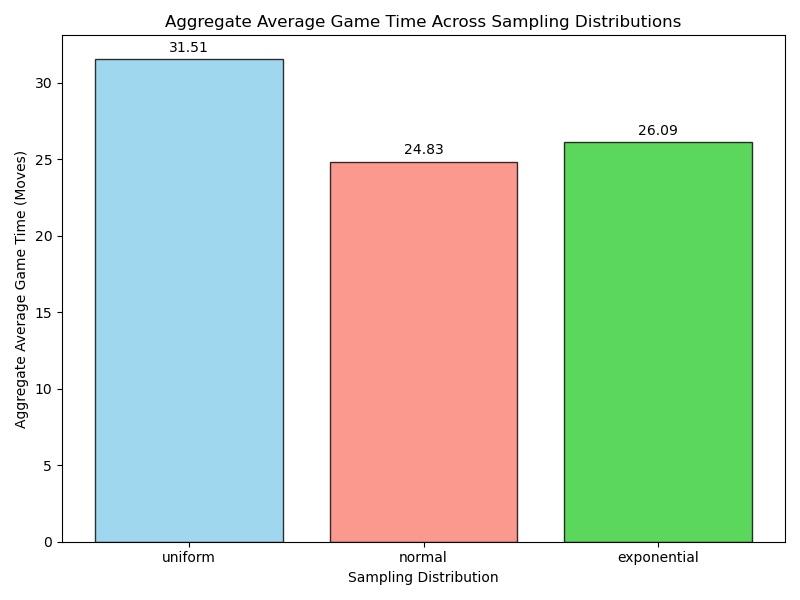
\includegraphics[width=0.5\textwidth]{"/home/ja1peg/Desktop/DissertationDocs/Dissertation/Chapter 2/withLength/FinalSampling/comparative_aggregate_average_game_times.png"} 
		\caption{Aggregated Averages of Game Time across the sampling distributions}
		\label{fig:sampling_dist_avg_times}
	\end{figure}
	
	Frequency distributions of game times for a fixed board layout under each sampling method (Fig. \ref{fig:sampling_dist_layout_dists}) reveal right-skewness across all three distributions, indicating that while most games finish within a moderate set of moves, outliers leading to longer games are possible. Exponential sampling exhibits the highest variability, possibly due to the prevalence of smaller entities and their random placement. Figure \ref{fig:sampling_dist_board_avg_times} (b) indicates that boards generated using exponential sampling consistently result in higher average game times compared to other methods. Figure \ref{fig:sampling_dist_board_avg_times} (a) shows that uniform distribution results in more consistently lower average game times across different board layouts, albeit with some boards exhibiting higher averages. Normal distribution displays the most variability across the boards played but with consistently low average game times and fewer outliers pushing game times upward.
	
	\begin{figure}[ht]
		\centering
		\subfloat[]{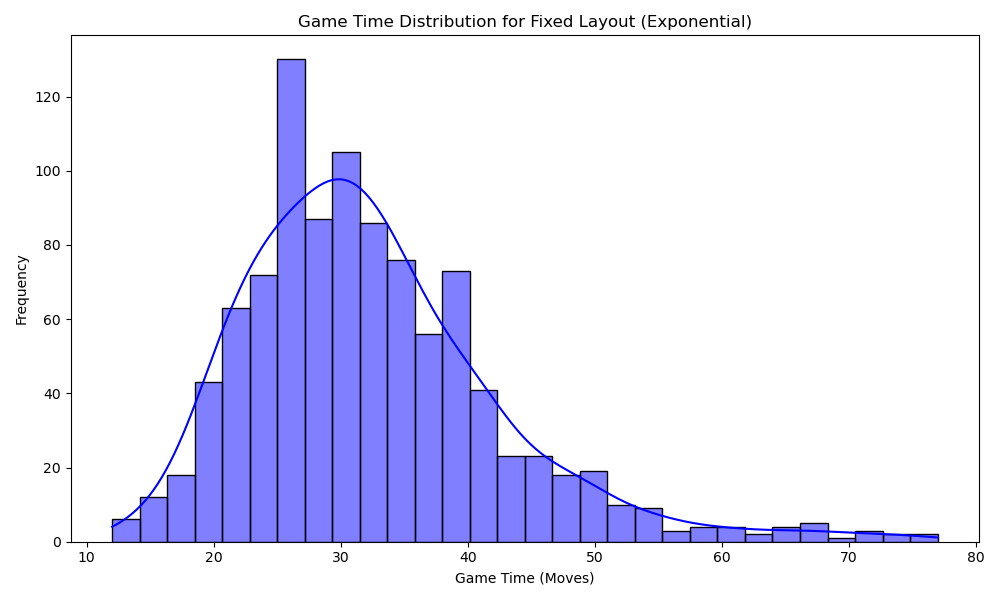
\includegraphics[width=0.3\textwidth]{"/home/ja1peg/Desktop/DissertationDocs/Dissertation/Chapter 2/withLength/FinalSampling/full_distribution_exponential.png"}} 
		\subfloat[]{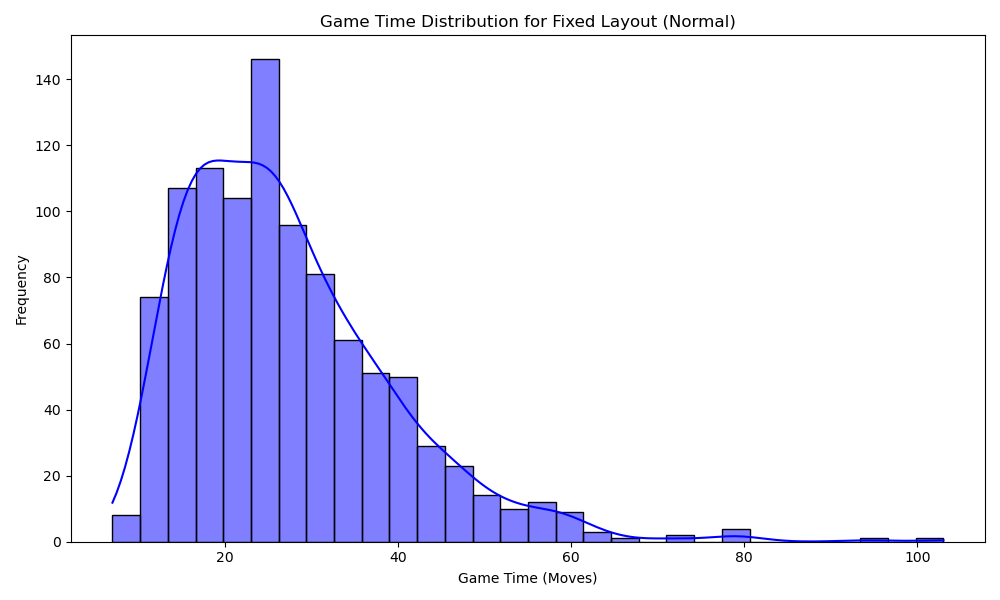
\includegraphics[width=0.3\textwidth]{"/home/ja1peg/Desktop/DissertationDocs/Dissertation/Chapter 2/withLength/FinalSampling/full_distribution_normal.png"}} 
		\subfloat[]{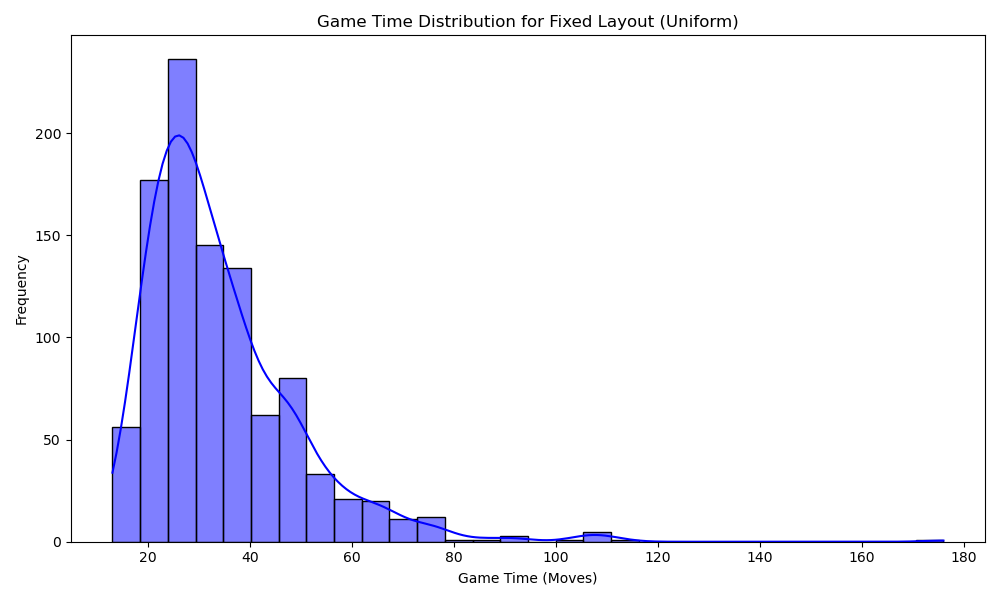
\includegraphics[width=0.3\textwidth]{/home/ja1peg/Desktop/DissertationDocs/Dissertation/Chapter 2/withLength/FinalSampling/full_distribution_uniform.png}} 
		\caption{Game Time Distributions for a Fixed Layout, by Sampling Method}
		\label{fig:sampling_dist_layout_dists}
	\end{figure}
	
	\begin{figure}[ht]
		\centering
		\subfloat[]{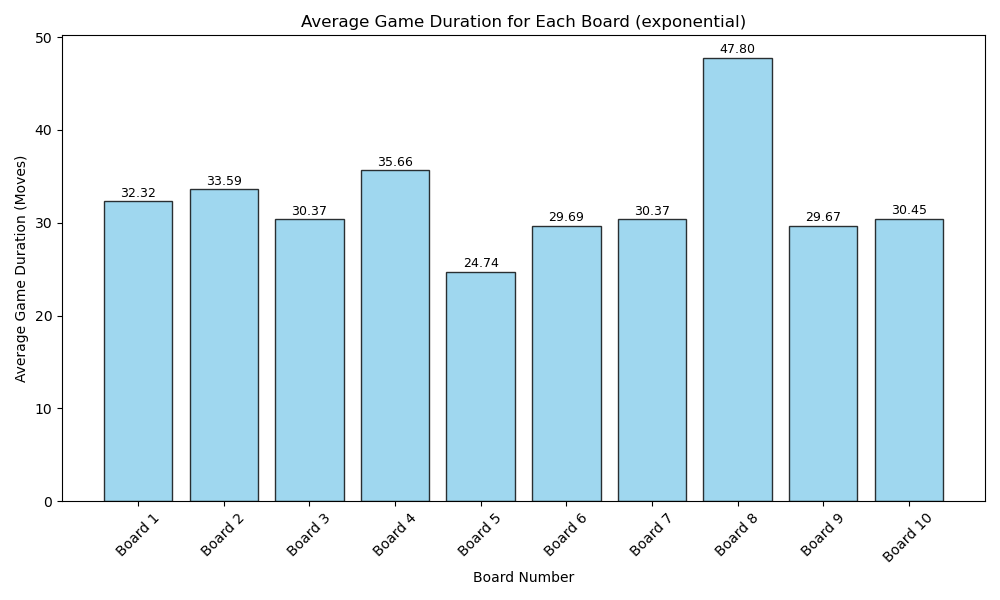
\includegraphics[width=0.45\textwidth]{"/home/ja1peg/Desktop/DissertationDocs/Dissertation/Chapter 2/withLength/FinalSampling/board_averages_exponential.png"}} 
		\subfloat[]{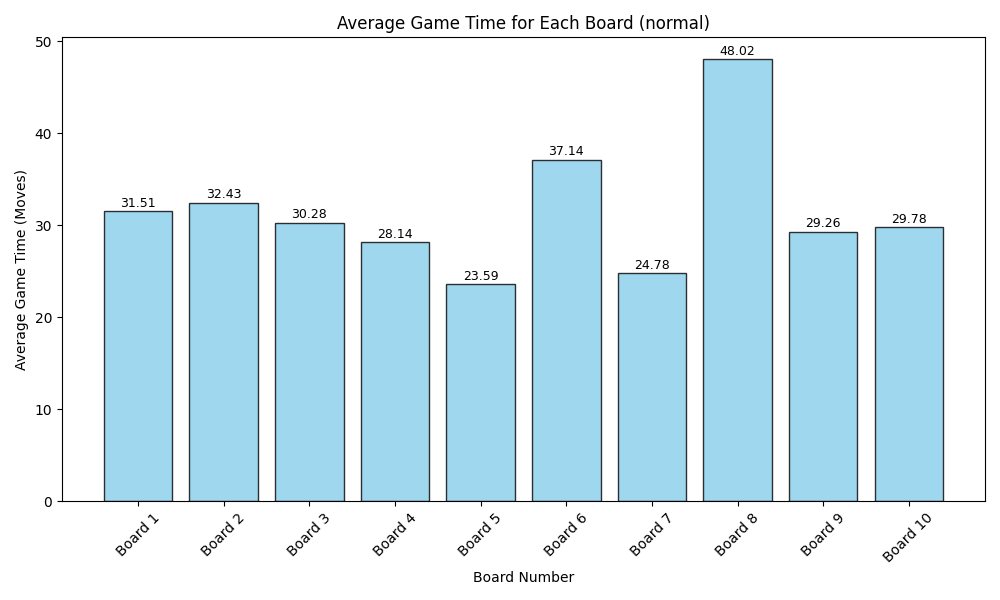
\includegraphics[width=0.45\textwidth]{"/home/ja1peg/Desktop/DissertationDocs/Dissertation/Chapter 2/withLength/FinalSampling/board_averages_normal.png"}}
		\linebreak
		\subfloat[]{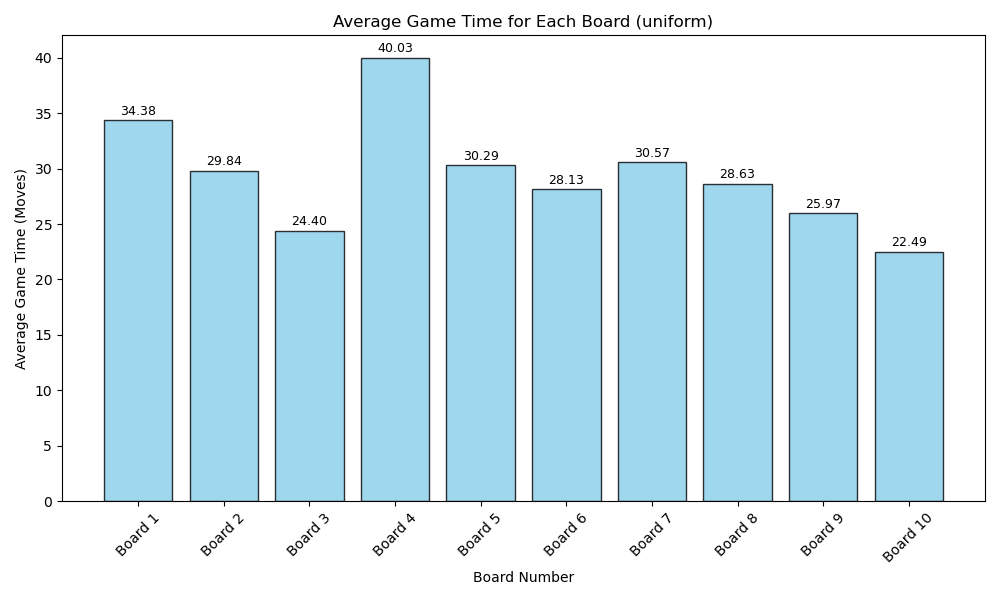
\includegraphics[width=0.45\textwidth]{"/home/ja1peg/Desktop/DissertationDocs/Dissertation/Chapter 2/withLength/FinalSampling/board_averages_uniform.png"}}
		\caption{Average Game Time for Each Board, by Sampling Distribution}
		\label{fig:sampling_dist_board_avg_times}
	\end{figure}
	
	
	\subsection{Randomly Generated Boards: Fixed Start and End Points}
	
	This section examines the effect of randomly generated snakes and ladders based on fixed start and end positions. Positions are generated while adhering to length constraints. This approach introduces greater variability compared to methods where lengths are predetermined. Figure \ref{fig:random_boards_avg_times} (a) illustrates average game times across 10 randomly generated boards. Each bar represents the average game time for a specific board, revealing significant variability in average game times across different board layouts, ranging from approximately 22 to 40 moves. Figure \ref{fig:random_boards_game_dist} (b) displays the frequency distribution of game times across all simulated games, indicating similar variability, as evidenced by random spikes in certain sections and the kernel density line. Certain boards, due to their specific configurations, present varying challenges and opportunities for the agent, leading to a wide range of game durations.
	
	\begin{figure}[ht]
		\centering
		\subfloat[]{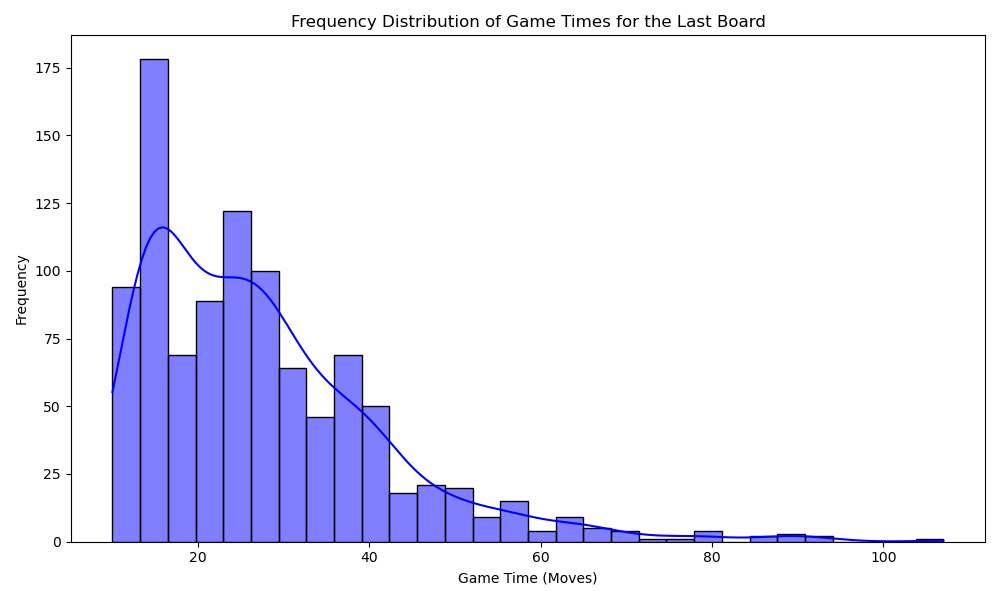
\includegraphics[width=0.45\textwidth]{"/home/ja1peg/Desktop/DissertationDocs/Dissertation/Chapter 2/withLength/RandomLength/approach_3_game_time_distribution.png"}}
		\subfloat[]{\includegraphics[width=0.45\textwidth]{"/home/ja1peg/Desktop/DissertationDocs/Dissertation/Chapter 2/withLength/RandomLength/approach\_3\_random\_points.png"}} 
		\caption{Analysis of Randomly Generated Boards}
		\label{fig:random_boards_avg_times}
		\label{fig:random_boards_game_dist}
	\end{figure}
	
	
	\section{Analysis}
	
	This chapter explores the impacts of both entity number and length ($L^S$ and $L^L$) on game dynamics in \textit{Snakes and Ladders}. By simulating games under systematically varied parameters across different approaches—static length assignment, statistical length sampling, and randomized start/end points, revealing several key insights.
	
	Firstly, variations in both the \textit{number} and \textit{lengths} of snakes and ladders significantly influence game duration and its variability. Increased numbers of snakes generally prolong games, while more ladders tend to shorten them. However, the relationship is not always linear, with thresholds and interactions between entity types playing a crucial role. For example, while simply increasing snake count does not always linearly increase game time, exceeding a certain density of snakes dramatically extends game duration. Conversely, the positive impact of ladders is more pronounced in mitigating the negative effects of high snake counts.
	
	Secondly, the method of assigning entity lengths introduces another layer of complexity. Deterministic length assignments provide a baseline for understanding game mechanics, while statistical sampling reveals how different length distributions affect game variability and average duration. Exponential distributions, favoring shorter lengths, tend to increase game time and variability, whereas normal distributions offer a more balanced outcome. Uniform distributions, in contrast, result in shorter, more predictable games. Randomly generated boards based on fixed start and end points introduce the highest degree of variability, highlighting the significant impact of entity placement on overall game dynamics.
	
	Thirdly, the presence of outliers and fluctuating trend lines across different board layouts underscores the significant influence of board layout itself. Strategic placement of snakes and ladders can create "traps" or "shortcuts," leading to substantial variations in game duration even within the same parameter configurations.
	
	These findings have valuable implications for game design and balancing. They demonstrate how adjusting the number and lengths of snakes and ladders can fine-tune game difficulty and duration. The choice of length assignment method—deterministic, sampled, or position-based—further allows designers to control the level of variability and unpredictability in gameplay. For games with mechanics similar to \textit{Snakes and Ladders}, these insights can inform the creation of engaging experiences with carefully calibrated challenge and playtime.
	
	Additionally, this chapter lays the groundwork for a more advanced analytical approaches. The observed complexities and probabilistic nature of \textit{Snakes and Ladders} dynamics suggest the utility of Markov models for deeper investigation. As the research moves forward, employing Markov models will allow to gain more nuanced insights into game mechanics, predict expected game durations for specific board configurations, and further quantify the elements that contribute to the overall player experience. 
	
	\chapter{Setting up a Markov Model}
	In this chapter, an analytical framework based on Markov chain theory to model the dynamics of Snakes and Ladders is utilised. This approach provides a rigorous method for quantifying game progression and predicting key metrics, such as the expected number of turns to reach the final board position. 
	
	\section{What are Markov Chains}
	A Markov chain is a mathematical system that experiences transitions from one state to another in a chain-like process. Its defining characteristic is the memoryless property: the probability of transitioning to the next state depends solely on the current state and not on the sequence of events that preceded it. In the context of Snakes and Ladders, each board position is treated as a state, and the outcome of a dice roll determines the probability of moving from one state to another.
	
	By adopting a Markov chain framework, the random nature of the game can be captured, where each dice roll is independent—and incorporate the special rules governing snakes and ladders. This model enables a transition beyond empirical simulation and derive analytical expressions for key performance measures, such as the average number of moves required to complete the game.
	
	\section{Fundamental Concepts}
	Before detailing the construction of our model, it is important to define several key concepts:
	\begin{enumerate}
		\item 	\textbf{States:} In our model, each tile on the board (from 0 to the board size) represents a state. The starting position is state 0, and the final position (the goal) is an absorbing state, meaning that once reached, no further transitions occur.
		\item \textbf{Transitions:} A transition is the movement from one state to another. In Snakes and Ladders, transitions occur as a result of dice rolls. Each roll yields one of six outcomes (with equal probability of 	$\frac{1}{6}$), which, when added to the current position, determine the next state.
		\item \textbf{Absorbing States: }An absorbing state is one that, once entered, cannot be left. In our game, the final tile is an absorbing state because the game terminates when the player reaches or exceeds it.
		\item \textbf{Memorylessness: }The Markov property implies that the probability of moving to a new state depends solely on the current state, not on how that state was reached. This simplifies the analysis, as the past history of the game does not need to be considered when determining future moves.
	\end{enumerate}
	
	\section{Constructing the Transition Matrix}
	The transition matrix is a square matrix $P$ of dimensions $(N+1)  \times (N+1)$ (where $N$ is the board size), and each entry $P(i,j)$ represents the probability of moving from state $i$ to state $j$ in one turn. $N_S$ and $N_L = 10$ and their lengths are randomly assigned using the fixed start and end points approach from Chapter 2.
	
	\subsection{Methodology}
	For each non-absorbing state (i.e. every state except tile 100):
	\begin{enumerate}
		\item \textbf{Dice Roll Outcomes:} The agent rolls a fair six-sided die. Each outcome, $k$ (where $1 \leq k \leq 6$), occurs with probability $\frac{1}{6}$
		\item \textbf{Movement Calculation:} The tentative new state is calculated by adding the dice roll $k$ to the current state $i$. If the tentative new state exceeds the board limits, the excess is subtracted from the final state. This ensures that the player remains on a valid tile.
		\item \textbf{Entity Adjustments:} If the resulting state corresponds to the head of a snake or the base of a ladder, the state is immediately updated to the corresponding tail or top, respectively.
		\item \textbf{Matrix Population:} For each dice outcome, the appropriate transition probability is added to the matrix entry corresponding to the final state after making all adjustments
	\end{enumerate}
	
	For the absorbing state (the final board position), the row in the matrix is set to have a probability of 1 for the remaining in that state, reflecting that no further moves occur once the goal is reached.
	
	For all non-absorbing states $i$:
	\[
	P(i, j) = \sum_{k=1}^{6} \frac{1}{6} \cdot \mathbf{1}\{ f(i,k) = j \}
	\]
	where $f(i,k)$ is the function that computes the new state after adding the dice roll $k$ to state $i$, applying reflection if necessary, and adjusting for any snake or ladder. The indicator function $\mathbf{1}\{\cdot\}$ equals 1 if the condition is met, and 0 otherwise.
	
\[
P(n, n) = 1 \quad \text{and} \quad P(n, j) = 0 \quad \text{for} \quad j \neq n.
\]

	This formulation guarantees that each row of the transition matrix sums to 1, thereby satisfying the properties of a stochastic matrix.
	
	\section{Expected Turns via the Fundamental Matrix}
	
	To determine the average number of moves required to reach the absorbing state from the starting state, we employ the concept of the \textit{fundamental matrix}.
	
	\subsection{Partitioning the Matrix}
	
	The transition matrix $P$ is partitioned into two segments:
	\begin{itemize}
		\item $Q$: The submatrix corresponding to the transient states (all states except the absorbing state).
		\item $R$: The submatrix describing transitions from transient states to the absorbing state.
	\end{itemize}
	
	\subsection{Fundamental Matrix Calculation}
	
	The fundamental matrix $N$ is computed as:
	\[
	N = (I - Q)^{-1}
	\]
	where $I$ is the identity matrix of the same dimension as $Q$. The entry $N(i, j)$ represents the expected number of times the process is in state $j$ when starting from state $i$ before absorption occurs.
	
	\subsection{Deriving Expected Turns}
	
	The expected number of turns $t$ required to reach the absorbing state from the initial state (state 0) is given by summing the entries in the first row of $N$:
	\[
	t = \sum_{j} N(0, j)
	\]
	This sum reflects the total expected visits to all transient states, effectively yielding the average number of turns needed to complete the game.
	
	\section{Steady-State Distribution in an Absorbing Chain}
	
%	While the primary interest in an absorbing Markov chain is the expected time to absorption, analysing the steady-state distribution can provide insight into the transient behaviour of the system. By iteratively multiplying an initial state vector by the transition matrix, one observes the evolution of the probability distribution over the states. Over a sufficiently large number of iterations, the state probabilities converge, highlighting the relative frequency of being in particular states before the game terminates.
	
	\section{Conclusion}
	
	
\end{document}